\documentclass[10pt,table,xcdraw]{article}
\usepackage[es-tabla]{babel}
\usepackage{parskip}
\usepackage[capitalise, noabbrev]{cleveref}
\crefname{table}{\spanishtablename}{\spanishtablename}



\title{
	\textbf{
		Desarrollo de un modelo fundacional estocástico basado en procesos Gaussianos para la clasificación de bioseñales EEG en el diagnóstico asistido del TDAH.
	}
	}
\author{
	Julián David Pastrana Cortés, M.Sc.
	}


\date{} % Carga el preámbulo
\begin{document}
	%%%%%%%%%%%%%%%%%%%%%%%%%%%%%%%%%% PORTADA %%%%%%%%%%%%%%%%%%%%%%%%%%%%%%%%%%%%%%%%%%%%
\vspace*{0.5cm}
\begin{center}
	\newcommand{\HRule}{\rule{\linewidth}{0.5mm}}
	\vspace*{-1.5cm}
	% \textsc{\huge Universidad Tecnológica\\ \vspace{5px} de Pereira}\\[1.5cm]
	% 
\includegraphics[width=0.2\textwidth]{imagenes/Logo_UTP.png}
	% \vspace{1.5cm}
	\textsc{\LARGE Informe de actividades en el marco del programa: \\ 
		\vspace{0.4cm}
		ALIANZA CIENTÍFICA CON ENFOQUE COMUNITARIO PARA MITIGAR BRECHAS DE ATENCIÓN Y MANEJO DE TRASTORNOS MENTALES RELACIONADOS CON IMPULSIVIDAD EN COLOMBIA
		}\\
	\vspace{2cm}
	\HRule \\[0.4cm]
	{ \bfseries Nombre: Julián David Pastrana Cortés }\\[0.4cm]
	{ \bfseries Contrato de servicios: 5551 }\\[0.4cm]
	\vspace{1.5cm}
	
\includegraphics[width=0.28\textwidth]{imagenes/LogoU.png}
	
\includegraphics[width=0.35\textwidth]{imagenes/logo_automatica.png}
	\HRule \\[1.5cm]
	\vspace{1.5cm}
	\vspace*{0.5cm}
	\textsc{\textbf{\Large Grupo de investigación en Automática } }\\
	\vspace{3.5cm} 
	\begin{center}
		{\large \today}
	\end{center}
\end{center}
\newpage
   % Carga la portada y otros elementos de layout
	
	\tableofcontents 
	\newpage
	
	\section{Información general del contrato}
	\begin{table}[H]
		\centering
		\begin{tabular}{>{\arraybackslash}m{8cm} >{\arraybackslash}m{6.5cm}}
			\toprule
			\textbf{Rol} & \vspace{2mm}Contratista - Estudiante de Doctorado\vspace{2mm}\\\hline
			\vspace{2mm}
			\textbf{Contrato de servicios No.}\vspace{2mm} & \vspace{2mm} 5551 de 2025\vspace{2mm}\\\hline
			\vspace{2mm}
			\textbf{Objeto del contrato} \vspace{2mm} & \vspace{2mm} Prestación de servicios profesionales para el Desarrollo de metodología de gamificación para entrenamiento de niños con trastornos de impulsividad ALIANZA CIENTÍFICA CON ENFOQUE COMUNITARIO PARA MITIGAR BRECHAS DE ATENCIÓN Y MANEJO DE TRASTORNOS MENTALES RELACIONADOS CON IMPULSIVIDAD EN COLOMBIA - ACEMATE MINCIENCIAS CONTRATO 790-2023 
			\vspace{2mm}\\\hline
			\textbf{Período del informe} & \vspace{2mm} 01 de marzo de 2025 al 31 de marzo de 2025\vspace{2mm}\\\hline
		\end{tabular}
	\end{table}
	
	\subsection{Descripción general de la vinculación}
	Como resultado de la vinculación se contribuye al alcance de el objetivo 3 del programa de investigación: ALIANZA CIENTÍFICA CON ENFOQUE COMUNITARIO PARA MITIGAR BRECHAS DE ATENCIÓN Y MANEJO DE TRASTORNOS MENTALES RELACIONADOS CON IMPULSIVIDAD EN COLOMBIA
	
	\subsection{Objetivo general}
	Desarrollar una metodología de gamificación para entrenamiento de niños con trastornos de impulsividad ALIANZA CIENTÍFICA CON ENFOQUE COMUNITARIO PARA MITIGAR BRECHAS DE ATENCIÓN Y MANEJO DE TRASTORNOS MENTALES RELACIONADOS CON IMPULSIVIDAD EN COLOMBIA - ACEMATE MINCIENCIAS CONTRATO 790-2023.
	
	
	\section{Metodología}
	Para llevar a cabo el objetivo general planteado, se plantean las siguientes etapas:
	\begin{itemize}
	\item Etapa 1: Revisión del estado del arte sobre gamificación y trastorno de impulsividad para identificar las mejores prácticas y metodologías existentes.
	\item Etapa 2: Desarrollo de una metodología preliminar de gamificación.
	\item Etapa 3: Redacción y sometimiento de un artículo de investigación en revista indexada, donde se exponga la metodología preliminar desarrollada.
	\item Etapa 4: Ampliación de la metodología preliminar de gamificación mediante el uso de Procesos Gaussianos.
	\item Etapa 5: Redacción y sometimiento de un artículo de investigación en revista indexada, donde se exponga la metodología final desarrollada.
	\item Etapa 6: Elaboración de un informe técnico final sobre el desarrollo y resultados de las actividades.
	\end{itemize}
	
	\section{Resultados}
	Versión final del estado del arte sobre modelos de detección del TDAH basados en modelos funcacionales y procesos Gaussianos redactado en una propuesta de doctorado. El documento se encuentra en la sección de anexos.
	
	Avance en el desarrollo de un modelo de inferencia basado en Procesos Gaussianos encadenados para la amplicación de la metodología de gamificación. Consiste en un conjunto de códigos en lenguaje Python.
	
	\section{Anexos}
% Include first page with a title overlay
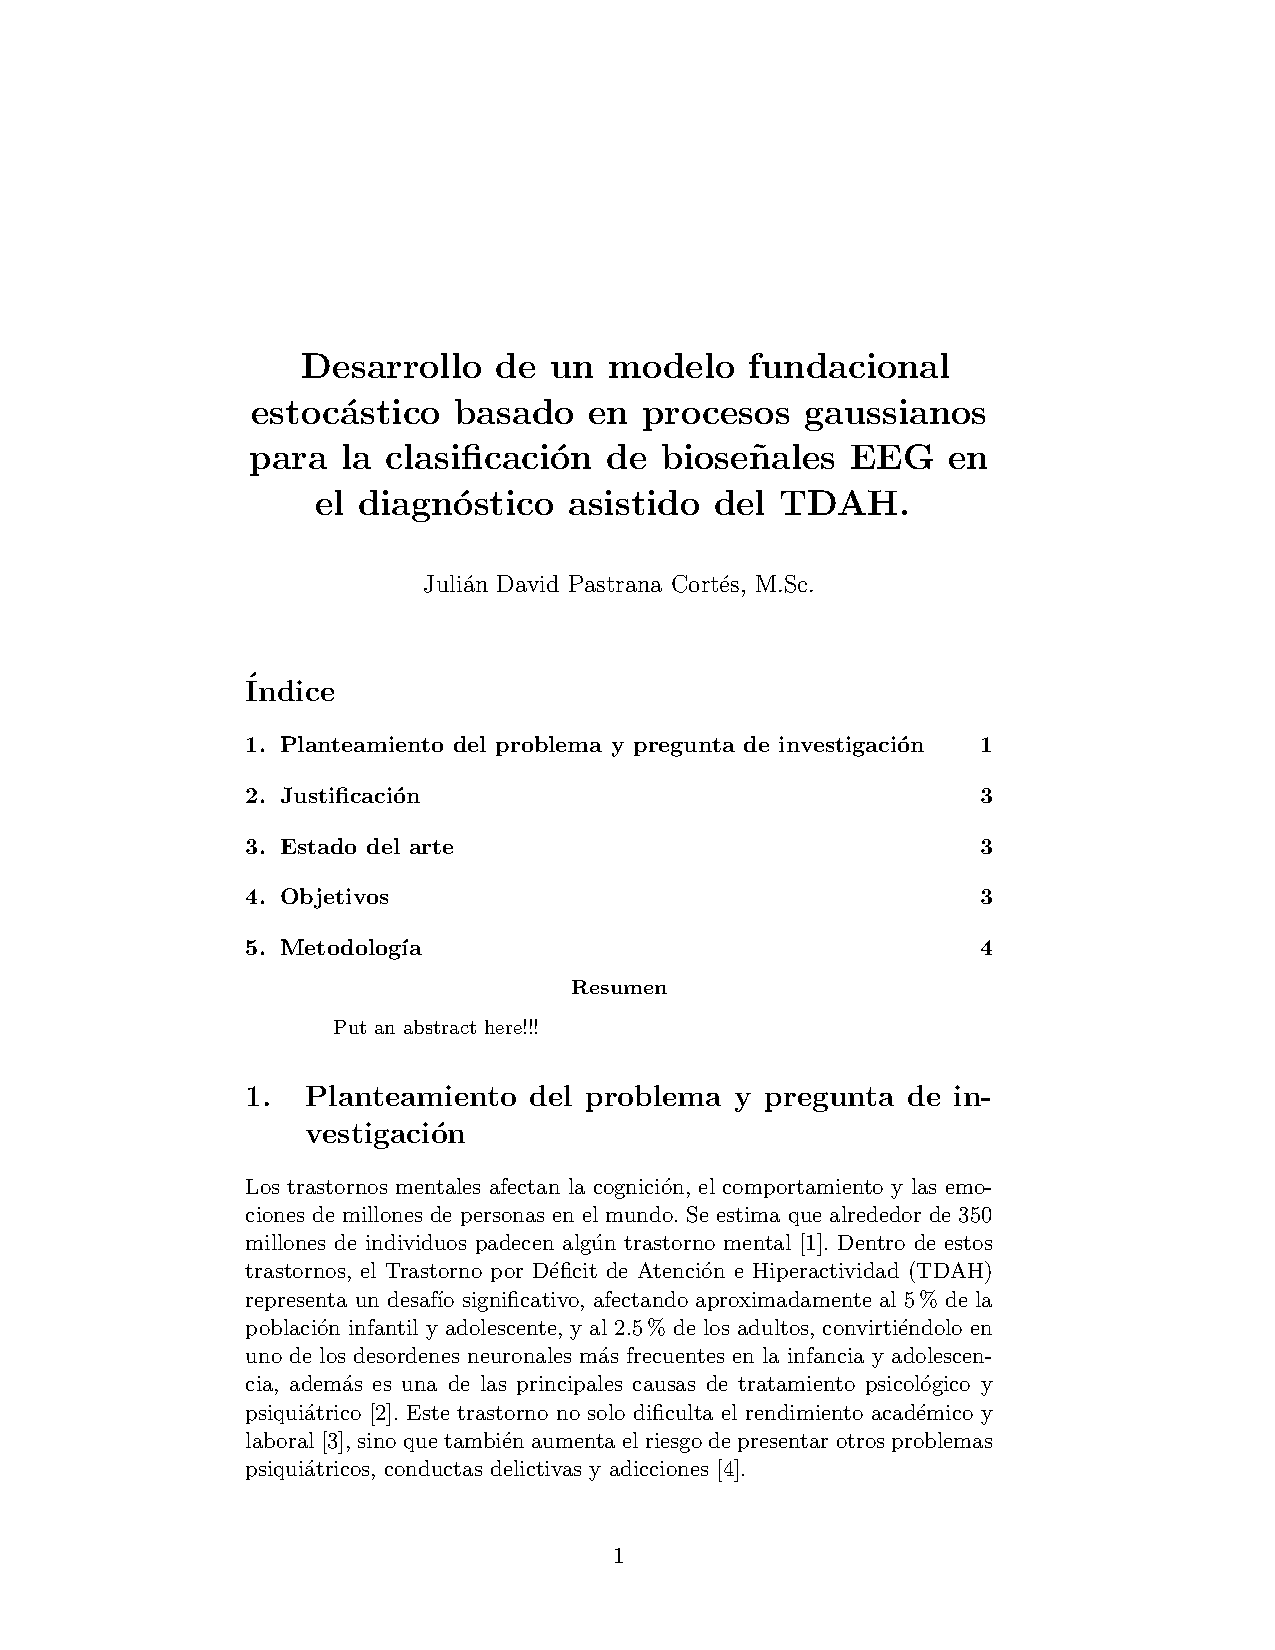
\includepdf[pages=1,
pagecommand={%
	\thispagestyle{plain}
		\Large\bfseries Propuesta doctorado
}
]{../propuesta_doctorado/main.pdf}
% Include remaining pages without any overlay
\includepdf[pages=2-last, pagecommand={}]{../propuesta_doctorado/main.pdf}

	\bibliographystyle{apalike}
%	\bibliography{refs}
	
\end{document}
